\documentclass[12pt]{article}

\author{Pietro Padovese}

\usepackage{graphicx}
\graphicspath{ {images/} }

\usepackage{amsmath}
\usepackage{booktabs}
\usepackage{changepage}
\usepackage{lipsum}
\makeatletter
\setlength{\@fptop}{0pt}
\makeatother
\usepackage[a4paper, total={6in, 8in}]{geometry}

\newcommand{\myparagraph}[1]{\paragraph{#1}\mbox{}\\}
\title{Stylised facts of the business cycle}

\begin{document}

\maketitle

\section{Point (a)}
Replicate Table 1 \textit{Cyclical Behaviour of the US Economy}\\\\


\begin{table}[htbp]
\begin{adjustwidth}{-1cm}{}
\begin{center}
\begin{tabular}{lrrrrrrrrrr}
\toprule
{} &   Sd\% &    t-4 &    t-3 &   t-2 &   t-1 &     t &   t+1 &   t+2 &    t+3 &    t+4 \\
\midrule
GDP          & 1.756 &  0.236 &  0.430 & 0.636 & 0.812 & 1.000 & 0.812 & 0.636 &  0.430 &  0.236 \\
CND          & 1.517 & -0.041 &  0.139 & 0.334 & 0.469 & 0.635 & 0.578 & 0.544 &  0.415 &  0.292 \\
CD           & 4.647 &  0.425 &  0.569 & 0.689 & 0.779 & 0.784 & 0.562 & 0.394 &  0.187 &  0.010 \\
Hours\_worked & 1.715 & -0.094 &  0.069 & 0.272 & 0.480 & 0.765 & 0.737 & 0.680 &  0.598 &  0.486 \\
Avg\_Hours    & 0.451 &  0.205 &  0.346 & 0.474 & 0.584 & 0.582 & 0.455 & 0.292 &  0.146 & -0.020 \\
Employment   & 1.459 & -0.174 & -0.029 & 0.165 & 0.372 & 0.679 & 0.696 & 0.683 &  0.639 &  0.555 \\
Productivity & 1.317 &  0.508 &  0.605 & 0.665 & 0.670 & 0.581 & 0.312 & 0.091 & -0.134 & -0.299 \\
Avg\_Wage     & 1.099 &  0.359 &  0.436 & 0.479 & 0.487 & 0.385 & 0.305 & 0.191 &  0.074 & -0.047 \\
\bottomrule
\end{tabular}
\end{center}
\end{adjustwidth}
\end{table}

\clearpage
Replicate Table 2 \textit{Business Cycle Statistics for the US Economy}
\begin{table}[h]
\centering
\begin{tabular}{lrrrr}
\toprule
{} &  Std\_dev &  Rel\_std\_dev &  Autocorr &  Corr\_output \\
\midrule
Y   &    1.765 &        1.000 &     0.814 &        1.000 \\
C   &    1.587 &        0.899 &     0.770 &        0.925 \\
I   &    6.590 &        3.733 &     0.833 &        0.867 \\
G   &    1.420 &        0.804 &     0.820 &        0.151 \\
w   &    1.099 &        0.622 &     0.856 &        0.382 \\
N   &    0.447 &        0.253 &     0.727 &        0.720 \\
Y/N &    1.476 &        0.836 &     0.800 &        0.978 \\
r   &    0.729 &        0.413 &     0.803 &       -0.054 \\
\bottomrule
\end{tabular}
\end{table}

\newpage
\section{Point (b)}
Verify whether or not the following business cycles facts hold today:\\\\
\textbf{Consumption is smoother than output}\\
Looking at Table 1 we can see that the standard deviation for the CND variable on non-durable consumptions (1.517) is slightly lower than the standard deviation of GDP (1.756), confirming that consumption is less volatile than output.  However, this difference is much less significant than that found by Cooley and Prescott.\\
If we look at the graph plotting the fluctuations in GDP and CND, we can indeed see that in the period prior to 1995 (the one examined by Cooley and Prescott), the fluctuations in GDP are much more pronounced than those in consumption. After 1995, on the other hand, these series follow a much more similar pattern, explaining the difference between the results found using more recent data. 

\begin{center}
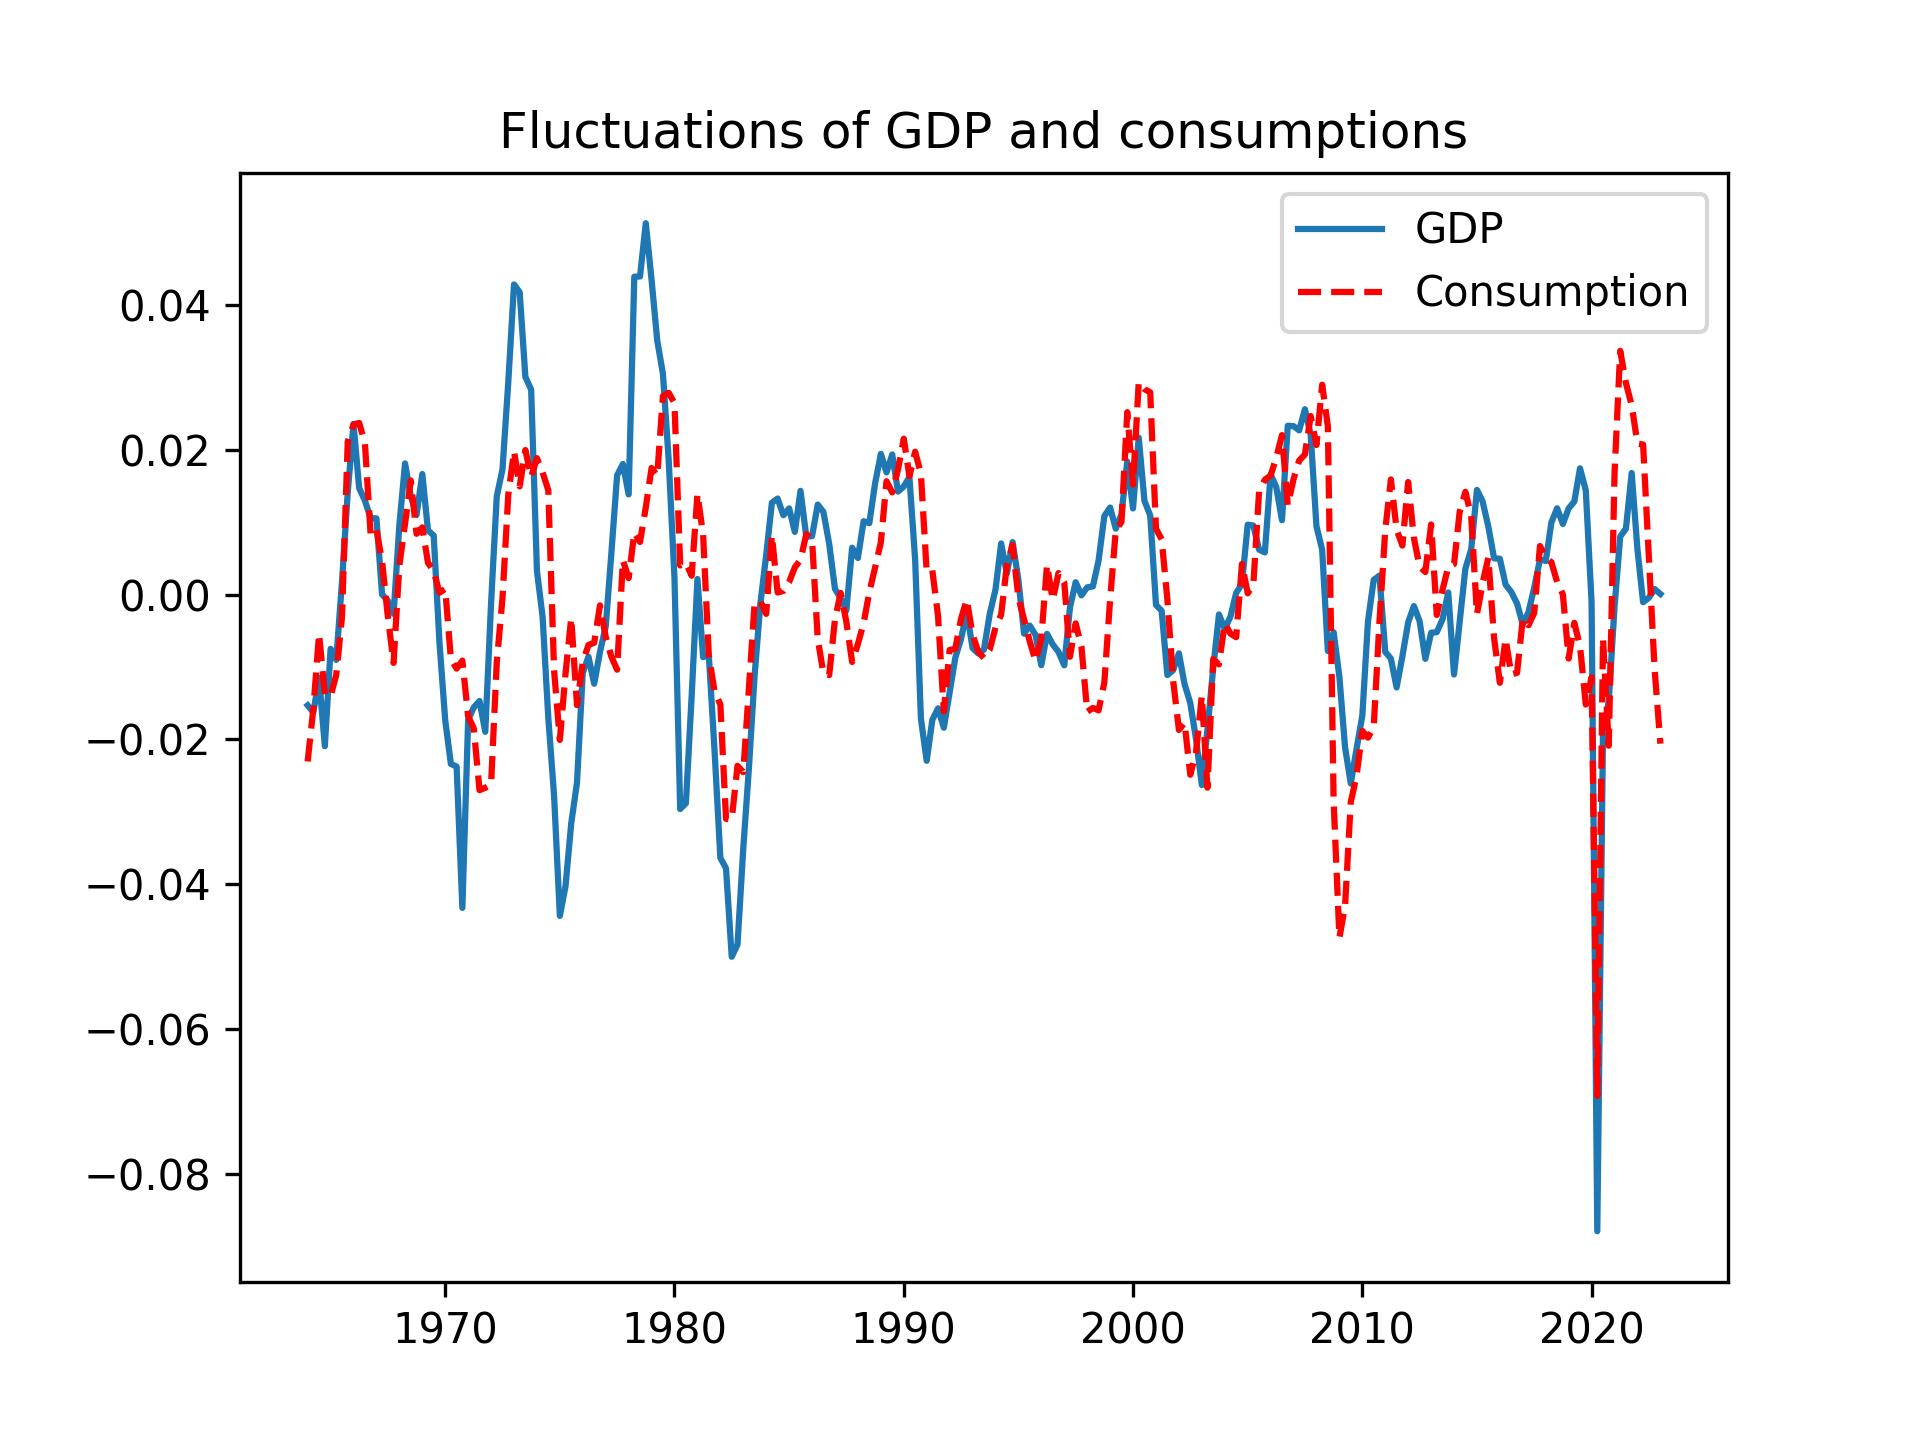
\includegraphics[width=0.8\textwidth]{cnd_gdp.jpg}
\end{center}
\textbf{Volatility in GDP is similar in magnitude to volatility in total hours}\\
Yes, in my data I found the volatility of GDP (1,756) and total hours (1,715) to be almost identical, even more than what Cooley and Prescott found. This result is explained by the fact that in periods of growth firms will use more hours to meet the increased demand for goods, and fewer hours in periods of decline.\\\\
\textbf{Volatility in employment is greater than volatility in avarage hours. Therefore most labour market adjustments operate on the extensive rather than intensive margin}\\
Yes, volatility in Employment (1.459), is much greater thant volatility in average hours (0.451)
This means that when companies need to use more manpower, instead of increasing the working hours of people already employed, they tend to hire new workers instead.\\\\
\textbf{Productivity is slighlty pro-cyclical}\\
If we look at the correlation of Productivity and output in table 1, we observe a value 0.581 and thus claim that productivity is pro-cyclical. If we broaden the time horizon by looking at the cross correlation between the two series and the fluctuation graph, we also notice that productivity, although procyclical, tends to anticipate output trends in some periods, suggesting the presence of some lag in the correlation. \\

\begin{center}
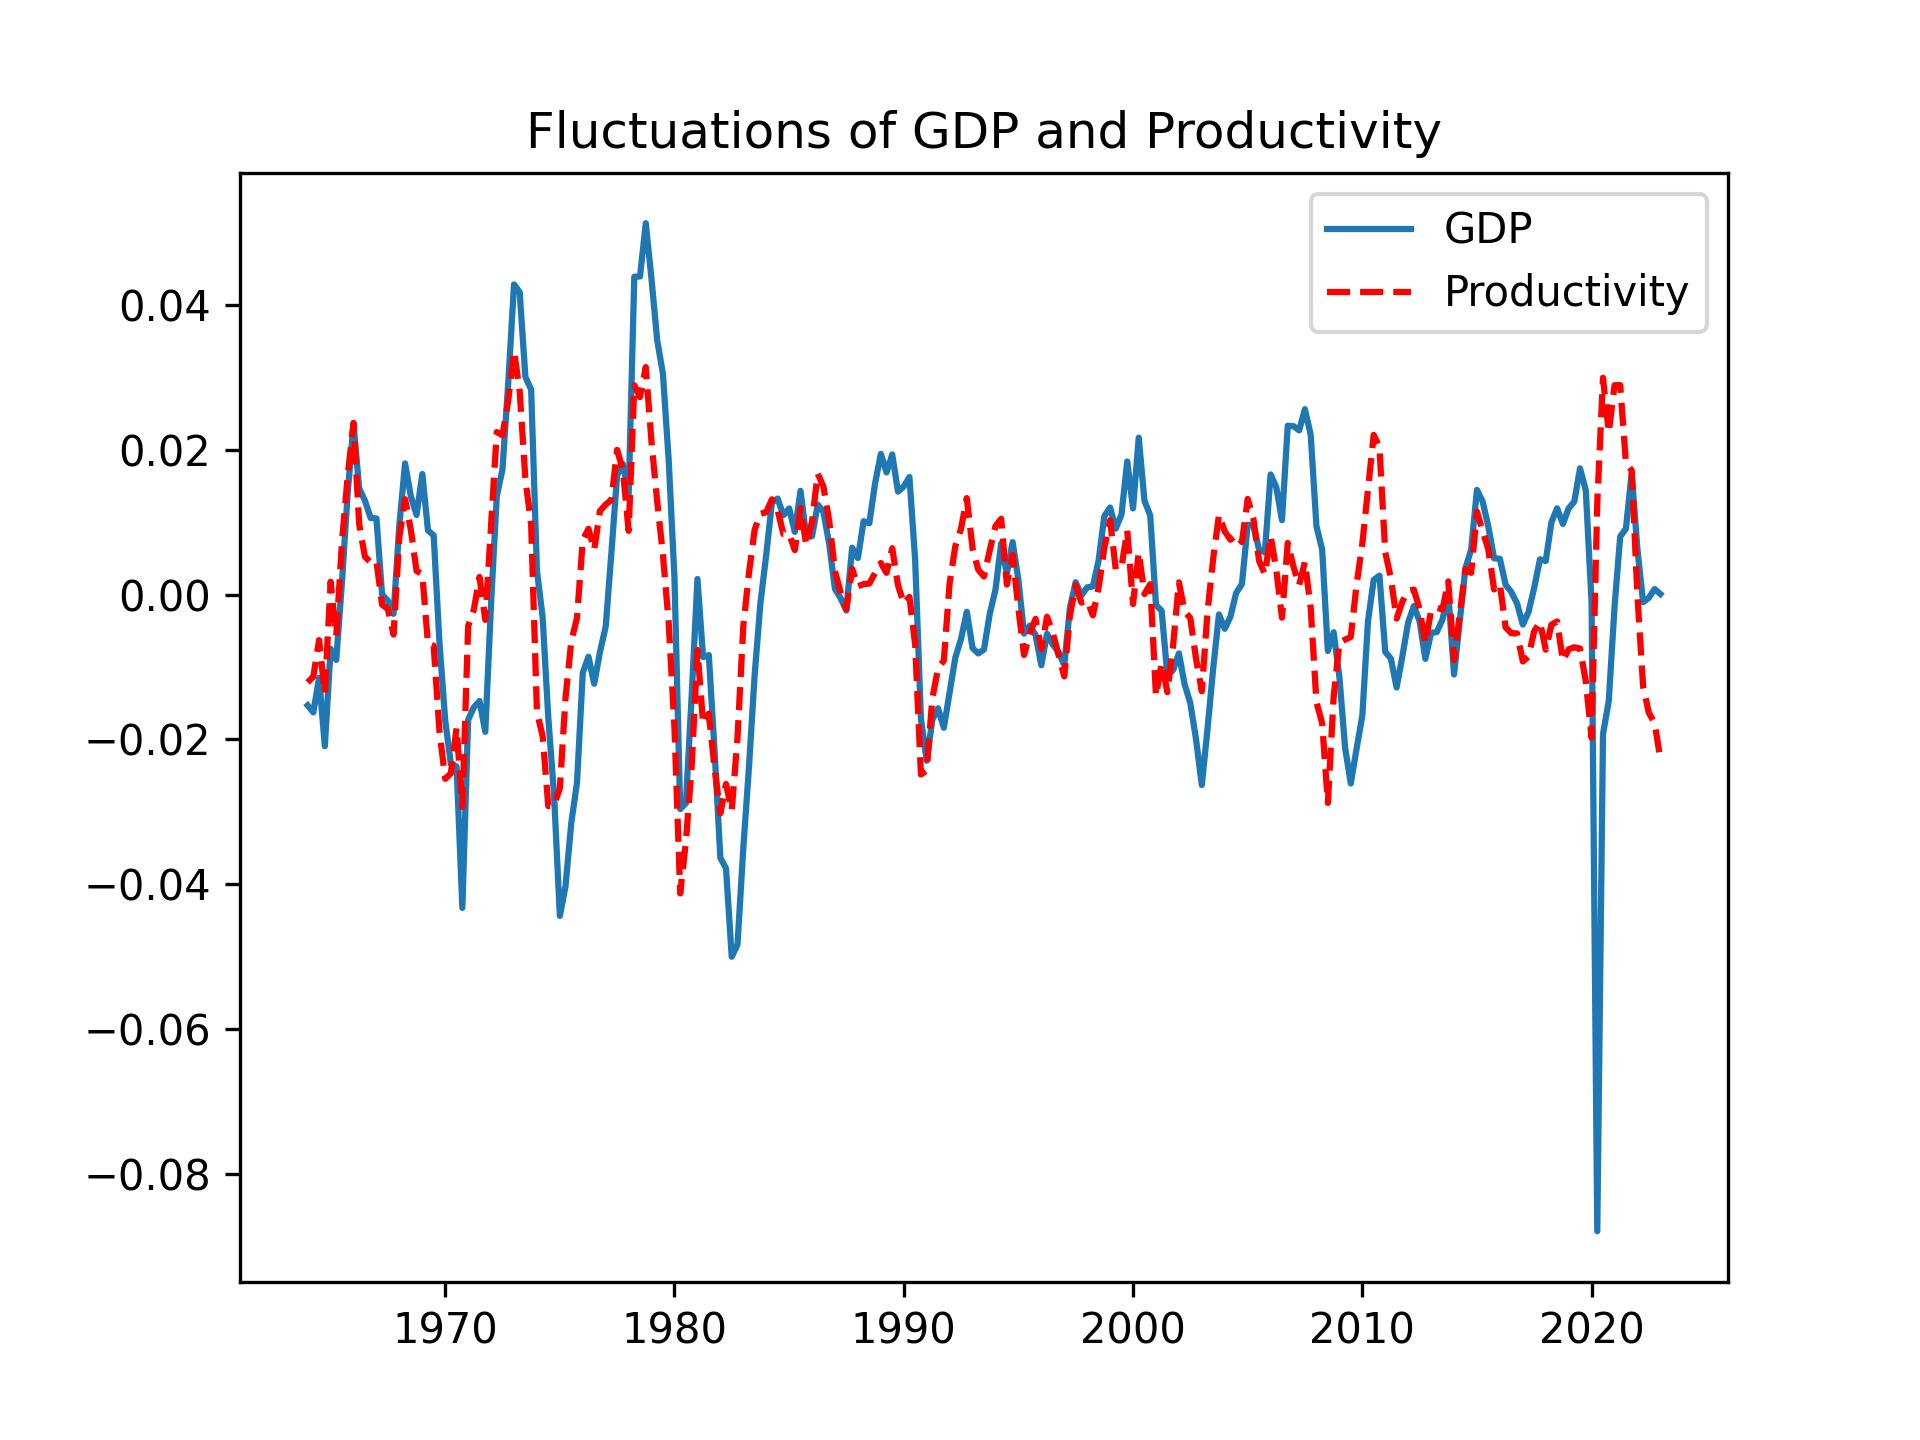
\includegraphics[width=0.8\textwidth]{productivity_gdp.jpg}
\end{center}
\textbf{Wages are less variable than productivity}\\
Yes, wages (1,099), appear to be less variable than productivity (1,317), a fact that can be explained by the difficulty of adjusting wages, as they are determined by social bargaining, as productivity changes.\\\\
\textbf{There is no correlation between wages and output}\\
From my analysis, contrary to the findings of Cooley and Prescott, I found a correlation between wages and output. Analyzing the graph, the data I used show a correlation even in the period prior to 1995. Explaining this difference would probably require a closer comparison of the data examined. 

\begin{center}
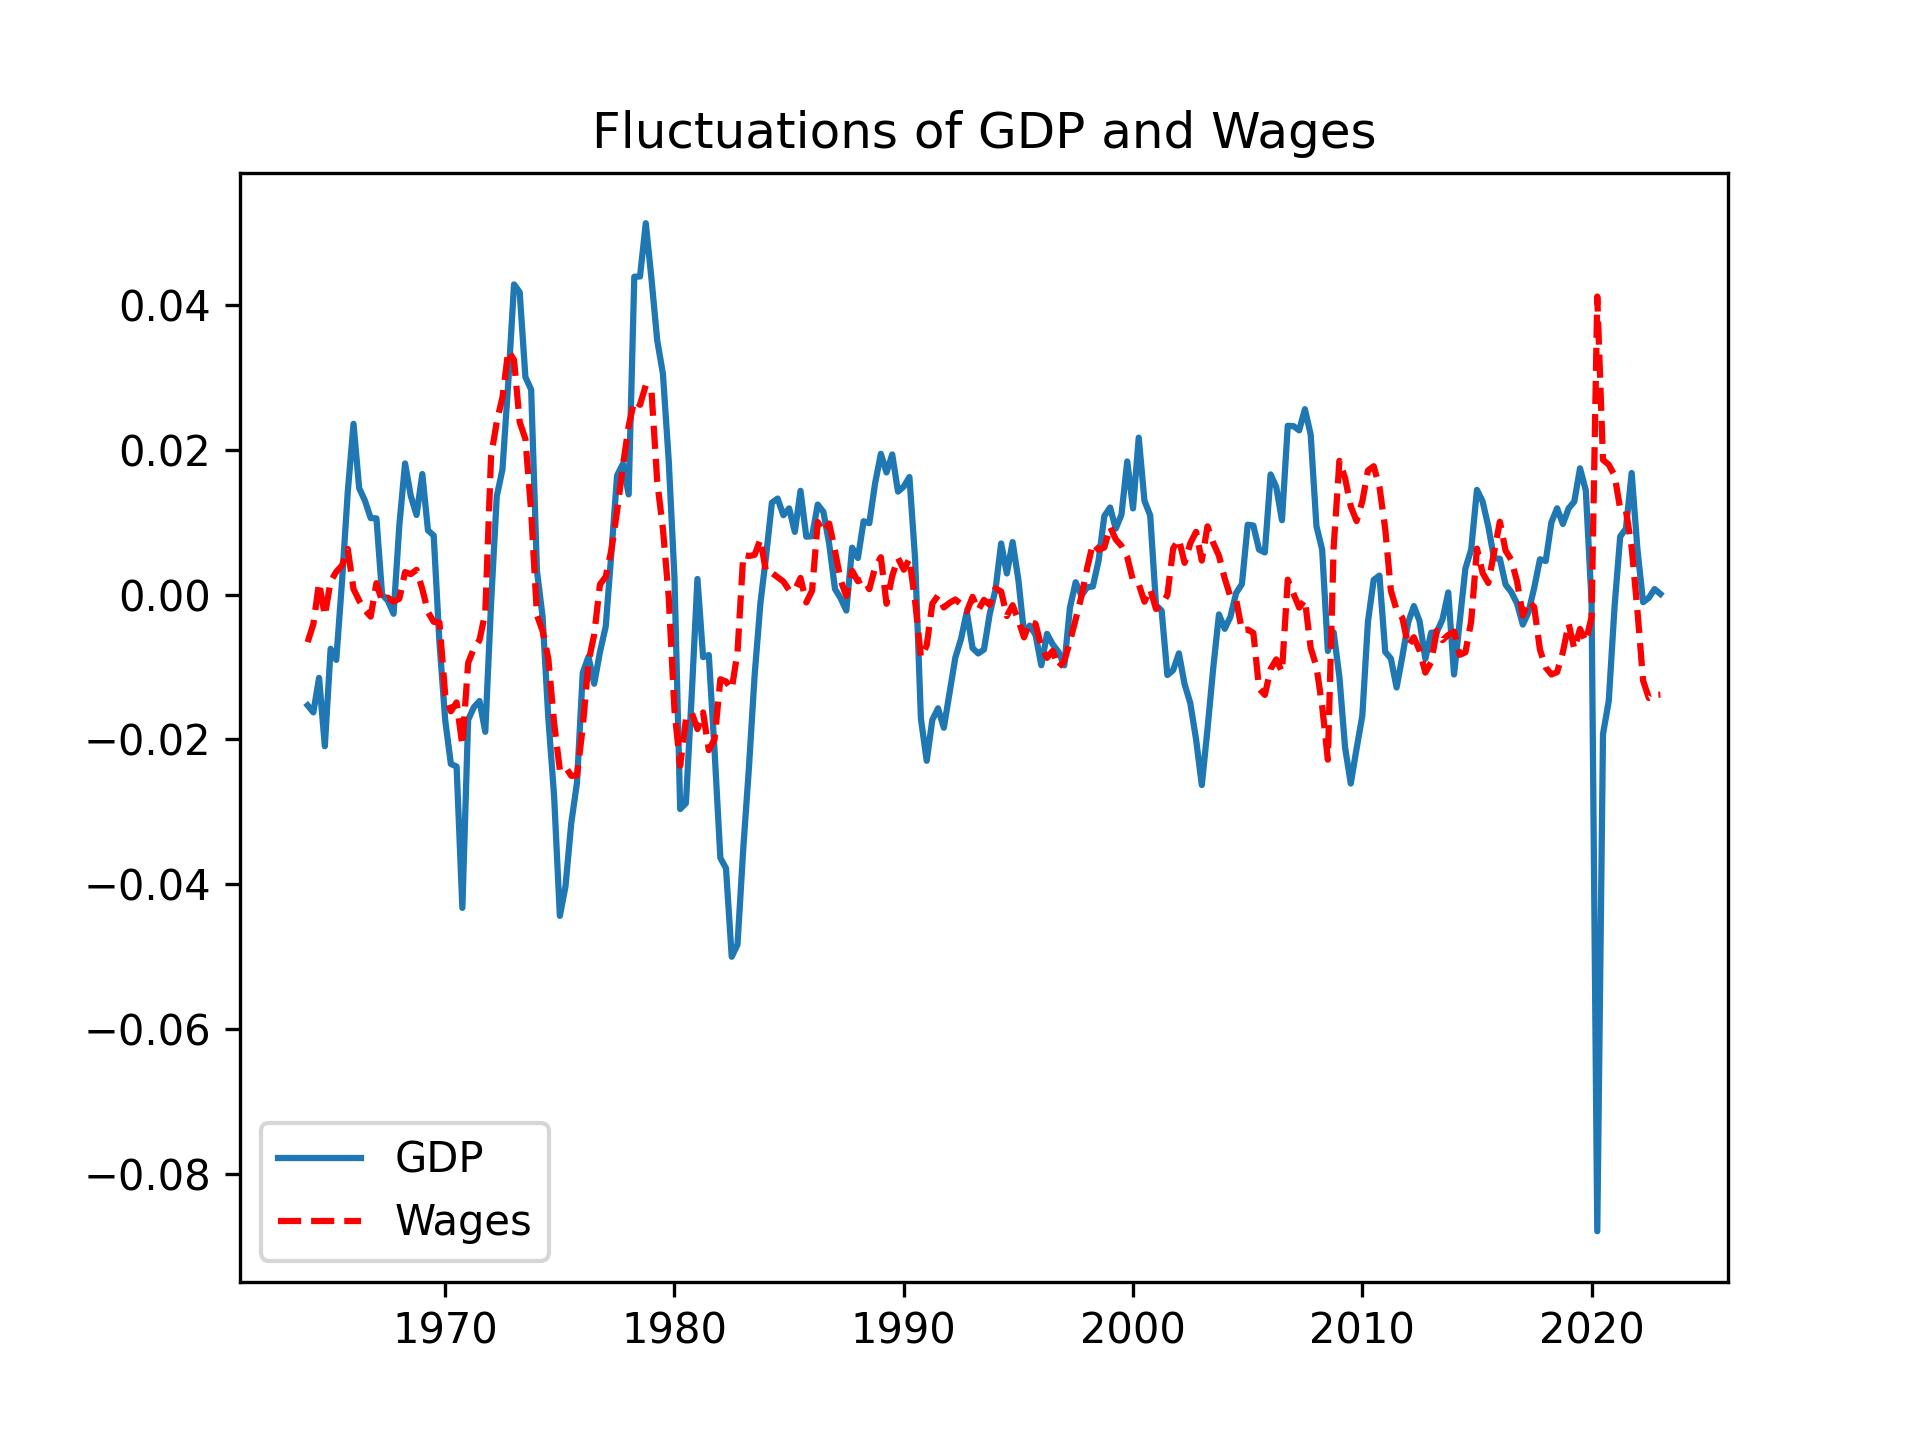
\includegraphics[width=0.8\textwidth]{wages_gdp.jpg}
\end{center}

\newpage
\section{Point (c)}

\textbf{Consumption of non-durables is less volatile than output}
See the first asnwer of point (b).\\\\
\textbf{Consumption of durables are more volatile than output}
Using the data from table 1 we can see that CD volatility (4.647) is indeed greater than volatility in output (1.756). Consumers are more influenced by the economic trend when they have to chose whether to buy durable goods, since they imply a higher impact on their income. \\\\
\textbf{Investment is three times more volatile than output}
I have found that investment is even more than three times more volatile than output (3.733). Firms during period of growth will have an excess of resources which they will use to make investments, but given that they are not necessary for their success in the short term, investment will be the first part of their budget to be cut off during downturns.\\\\
\textbf{Government expenditures are less volatile than output}
Yes, government expenditures (1.420) are less volatile than output (1.765). We need to consider that a large part of government expenditures are fixed amounts that are renewed every year and so they are independent from the economic trend.\\\\
\textbf{Total hours worked are about the same volatility as output}
See answer 2 of point (b)\\\\
\textbf{Employment is as volatile as output, while hours per worker are much less volatile than output}
Yes, Employment is almost as volatile as output, while hours per worker are much less volatile. As already discussed this means that in period of growth, firms tend to hire more workes than increase the hours of people already employed. \\\\
\textbf{Labour productivity is less volatile than output}
Yes, we can observe that labour productivity (1.476) is less volatile than output (1.765)\\\\

\newpage

\section*{Sources}
FRED's dataset library was used as the primary data source.\\
A dataset made available by the Bureau of Labor Statistics was used as a secondary source, particularly for the total number of hours worked and the level of employment. \\\\
One of the problems with some of the series was that data of real values going sufficiently far back in time were not available on FRED, where instead past values were present for their nominal equivalent. For this reason, I decided to download all the series at their nominal value and then apply the same conversion to all of them using the CPI. Since I was not aware of the method used by FRED for their conversions, I preferred this approach in order to have more consistency between the series. \\\\
What follows is the list of variables used extracted from FRED dataset, showing in bold the name associated with them within the exercise, their code and name of FRED dataset:
\begin{itemize}
\item \textbf{GDP}, \textit{GDP}, "Gross Domestic Product".
\item \textbf{CND}, \textit{PCND}, "Personal Consumption Expenditures: Nondurable Goods".
\item \textbf{CD}, \textit{PCDG}, "Personal Consumption Expenditures: Durable Goods".
\item \textbf{Avg\textunderscore Hours}, \textit{AWHNONAG}, "Average Weekly Hours of Production and Nonsupervisory Employees, Total Private", from "Current Employment Statistics (Establishment Survey)" \textsuperscript{1}, table: "Average weekly hours and overtime of production and nonsupervisory employees on private nonfarm payrolls by industry sector, Seasonally adjusted". 
\item \textbf{Avg \textunderscore Wage}, \textit{AHETPI}, "Average Hourly Earnings of Production and Nonsupervisory Employees, Total Private", from \textsuperscript{1}, table: "Avergae hourly and weekly earnings of production and nonsupervisory employees on private nonfarm payrolls by industry sector, Seasonally adjusted. 
\item \textbf{Y}, \textit{A939RC0Q052SBEA}, "Gross domestic product per capita".
\item \textbf{C}, \textit{A796RC0Q052SBEA}, "Personal consumption expenditures per capita: Goods: Nondurable goods".
\item \textbf{I}, \textit{GDPI}, "Gross Private Domestic Investment" (divided by the variable Pop to otbain the per capita value).
\item \textbf{G}, \textit{GCE}, "Government consumption expenditures" (divided by the variable Pop to otbain the per capita value).
\item \textbf{pop}, \textit{POPTHM}, "Population".
\end{itemize}
From the file "total-economy-hours-employmnet.xls", provided by BLS I have used the series: 
\begin{itemize}
\item \textbf{Hours worked}.
\item \textbf{Employment}.
\end{itemize}


\end{document}


